%%%%%%
% $Beschreibung: Frontblende $
% $Autor: ter Veen $
% $Datum: 15.06.2024 $
% $Version: 2 $
% $Pfad: SchrittmotorArduino/Manual/Tikz/Frontblende.tex $
%
%%%%%%

	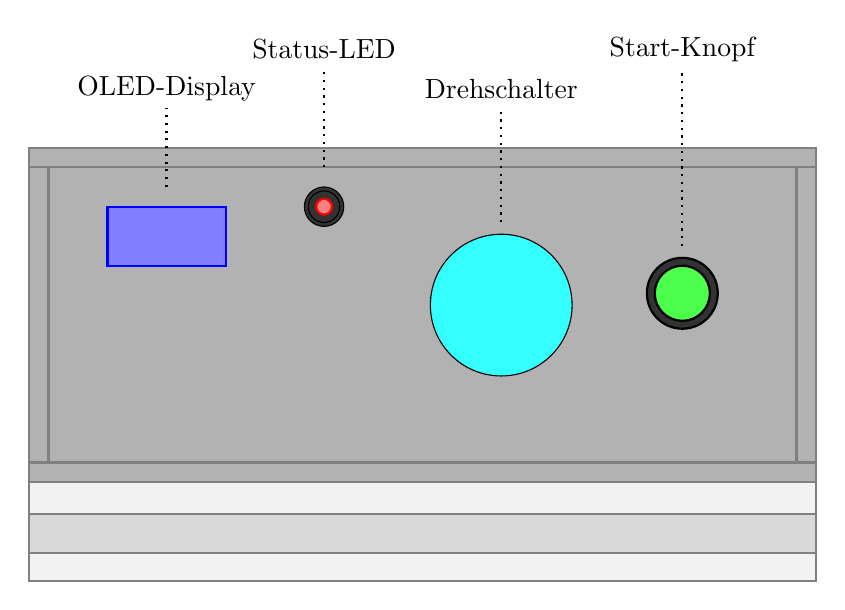
\begin{tikzpicture}
		%Gehäusedeckel
		\draw[gray, thick, fill=gray!60] (2,7) rectangle (12,7.25);
		
		% Gehäusemantel
		\draw[gray, thick, fill=gray!60] (2,3) rectangle (12,7);
		\draw[gray, thick, fill=gray!60] (2,3.25) rectangle (2.25,7);
		\draw[gray, thick, fill=gray!60] (11.75,3.25) rectangle (12,7);
		
		%Gehäuseboden
		\draw[gray, thick, fill=gray!60] (2,3) rectangle (12,3.25);
		
		% Alu-Profil
		\draw[gray, thick, fill=gray!10] (2,1.75) rectangle (12,3);
		\draw[gray, thick, fill=gray!30] (2,2.1) rectangle (12,2.6);
		
		% OLED-Display
		\draw[blue, thick, fill=blue!50] (3,5.75) rectangle (4.5,6.5);
		
		% Drehschalter
		\definecolor{cyan1}{rgb}{0 1 1};
		\draw[black, thin, fill=cyan1!80] (8,5.25) circle (0.9);
		
		% Status-LED
		\draw[black, thin, fill=black!80] (5.75,6.5) circle (0.25);
		\draw[black, thin, fill=black!80] (5.75,6.5) circle (0.2);
		\draw[red, thick, fill=red!50] (5.75,6.5) circle (0.1);
		
		% Start-Knopf (Button)
		\draw[black, thick, fill=black!80] (10.3,5.4) circle (0.45);
		\draw[black, thick, fill=green!70] (10.3,5.4) circle (0.35);
		
		% Punkt-Linien für Labels
		\draw[dotted, thick] (3.75,6.75) -- (3.75,7.75); % OLED-Display
		\draw[dotted, thick] (5.75,7) -- (5.75,8.25); % Status-LED
		\draw[dotted, thick] (8,6.3) -- (8,7.75); % Drehschalter
		\draw[dotted, thick] (10.3,6) -- (10.3,8.25); % Start-Knopf
		
		% Labels
		\node[] at (3.75,8) {OLED-Display};
		\node[] at (5.75,8.5) {Status-LED};
		\node[] at (8,8) {Drehschalter};
		\node[] at (10.3,8.5) {Start-Knopf};
	\end{tikzpicture}